\documentclass[12pt,a4paper,twoside]{article}
\usepackage[utf8]{inputenc}
\usepackage[spanish]{babel}
\usepackage{amsmath}
\usepackage{amsfonts}
\usepackage{amssymb}
\usepackage{graphicx}
\usepackage[left=2cm,right=2cm,top=2cm,bottom=2cm]{geometry}
\author{Yoleivys Delgado}
\title{\textbf{Movimiento de la Tierra y La Luna alrededor del Sol}}
\begin{document}
\maketitle
El movimiento traslacional de la tierra, es la trayectoria a lo largo de la cual la Tierra viaja alrededor del sol. La distancia promedio entre la tierra y el sol es de $149,000.000 Km$ y una orbita completa toma alrededor de 365.26 días y el movimiento traslacion de la luna alrededor de la tierra es realizado en 27.3 días aproximadamente.\\
Para la realización de este práctica supondremos que la tierra gira alrededor del sol con un \textbf{movimiento circular uniforme } a adistancia fija del sol de $R = 1.49 . 10^{8} Km $ y la luna gira alrededor de la tierra igualmente con un movimiento circular uniforme a una distancia fija de un decimo de la distancia del la tierra al sol.
La grafica optenida de esta practica como los codigos fortran y gnuplot son mostrados en las figuras (\ref{fig:figura1}),(\ref{fig:figura2}) y (\ref{fig:figura3}) . 

\begin{figure}[h]
\centering
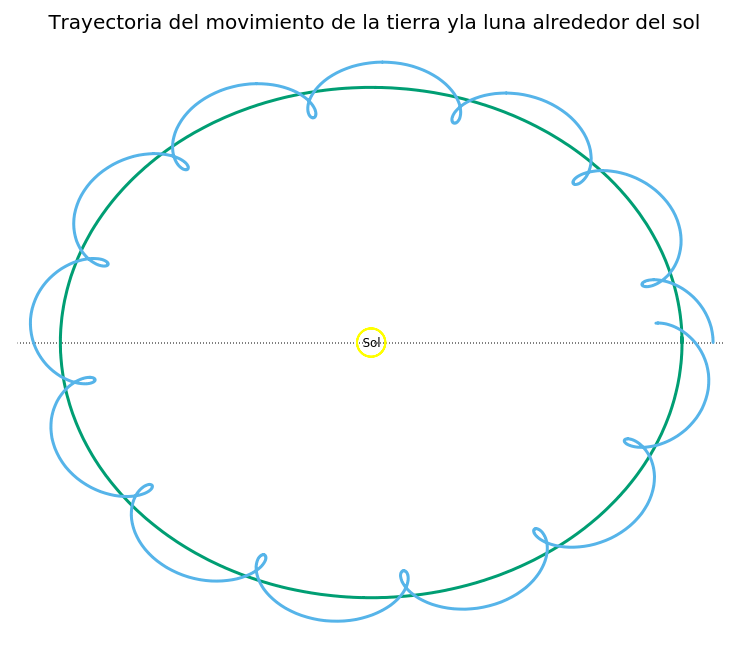
\includegraphics[width=10cm]{imagen.png} 
\caption{Trayectorias del movimiento de la Tierra y la Luna alrededor del Sol}
\label{fig:figura1}
\end{figure}

\newpage
\begin{figure}[h]
\begin{verbatim}
set title 'Trayectoria del movimiento de la tierra yla luna alrededor del sol'
set title font ",15" norotate
set style data lines      # Todas las graficas las pone con lineas
set xzeroaxis
unset key
unset border
unset xtics
unset ytics
set xrange [-170000000.0:170000000.0]
set yrange [-170000000.0:170000000.0]
set label 1 "Sol" at 0.0, 0.0 center front
plot "TierraLuna.txt" using 1:2 ls 2 lw 3,\
"TierraLuna.txt" using 3:4  ls 3 lw 3,\
"Sol.txt" using 2:3 with circles lw 2 lc rgb "yellow"
\end{verbatim}
\caption{Codigo gnuplot de la gráfica de la figura 1}
\label{fig:figura2}
\end{figure}

\begin{verbatim}
Subroutine posicion (Ang1,Ang2,x_tierra, y_tierra, x_luna, y_luna)
  implicit none
  
  double precision ,intent (in)::Ang1, Ang2
  double precision , intent (out)::x_luna, y_luna
  double precision ,  intent (out)::x_tierra, y_tierra
  
  ! variables locales 
  double precision, parameter :: R1=1.496d8          ! distancia entre la tierra y el sol
  double precision, parameter :: R2=1.496d7       !  distancia entre la tierra y la luna
     
  x_tierra = R1*dcos(Ang1)
  y_tierra = R1*dsin(Ang1)
  x_luna = R1*dcos(Ang1) + R2*dcos(Ang2)
  y_luna = R1*dsin(Ang1) + R2*dsin(Ang2)

end subroutine posicion
\end{verbatim}

\begin{figure}[h]
\begin{verbatim}
program movimiento
  !Este programa calcula la trayectoria de la tierra alrededor del sol
  ! y el de la luna alrededor de la tierra
  
  implicit none
  integer :: i
  integer, parameter:: ntime = 8800
  double precision  ::xpos_tierra, ypos_tierra
  double precision  ::xpos_luna, ypos_luna
  double precision, parameter :: pi=3.14159d0
  double precision, parameter ::T_tierra =8.766d3, T_luna =6.56d2 
  double precision :: AngTierra, AngLuna
  double precision, dimension(0:ntime):: xt, yt, xl, yl, dt

  open (1, file='TierraLuna.txt', status= 'unknown')
 
 do i=0,ntime,12
     
     dt(i) = dble (i)
     
     ! intervalo de ángulo tierra
    AngTierra = (2.0d0*pi*dt(i))/T_tierra

     ! intervalo de ángulo tierra
    AngLuna = (2.0d0*pi*dt(i))/T_luna
     ! llamando subroutina 

    call posicion (AngTierra, AngLuna,xpos_tierra,ypos_tierra,xpos_luna,ypos_luna)
    
    xt(i)=xpos_tierra
    yt(i)=ypos_tierra
    xl(i)=xpos_luna
    yl(i)=ypos_luna
    
     write (1,*)   xt (i), yt (i), xl (i), yl (i)
end do
  close (1)

end program movimiento

!************************************************************************************
   
\end{verbatim}
\caption{Codigo gnuplot de la gráfica de la figura 1}
\label{fig:figura3}
\end{figure}
\end{document}
